\documentclass[11pt,a4paper]{article}
\usepackage[latin1]{inputenc}
\usepackage{amsmath}
\usepackage{microtype}
\usepackage[none]{hyphenat}
\usepackage{verbatim}
\usepackage{amsfonts}
\usepackage{amssymb}
\usepackage{enumitem}
\renewcommand{\familydefault}{\sfdefault}
\usepackage{mathpazo}
\renewcommand{\rmdefault}{put}
\usepackage{enumitem}
\usepackage[dvipsnames,svgnames]{xcolor}
\usepackage{tkz-euclide}
\usetkzobj{all}
\usepackage{graphicx}
\usepackage{tikz} 	
\usepackage{adjustbox}
\usepackage{multicol}
\usepackage{lipsum}
\usepackage[left=0.7cm,right=1cm,top=1cm,bottom=1.5cm]{geometry}
\usepackage{cancel} \usepackage{xcolor}
\usepackage{tcolorbox}
\usetikzlibrary{decorations.pathmorphing,patterns}
\usetikzlibrary{decorations.pathreplacing,calc}
 \newcommand\coret[2][red]{\renewcommand\CancelColor{\color{#1}}\cancel{#2}}
\SetLabelAlign{Center}{\hfil\makebox[1.0em]{#1}\hfil}

%%_------= solusi


% Set this =0 to hide, =1 to show

% Set this =0 to hide, =1 to show
\newtcolorbox{mybox}[1][] { colframe = blue!10, colback = blue!3,boxsep=0pt,left=0.2em, coltitle = blue!20!black, title = \textbf{jawab}, #1, } 

%---------- kunci (jika 1 ) muncul
\def\tampilkunci{1}
\newcommand{\hide}[1]{\ifnum\tampilkunci=1
%
\begin{mybox}
 #1
\end{mybox}
%
\vspace{\baselineskip}\fi\ifnum\tampilkunci=0
%
\vspace{2cm}
%
\fi}



\newcommand*\cicled[1]{\tikz[baseline=(char.base)]{\node[white, shape=circle, fill=red!80,draw,inner sep=0.5pt](char){#1};}}

\newcommand*\kunci[1]{\ifnum\tampilkunci=1
%
\tikz[baseline=(char.base)]{\node[red, shape=circle,draw,inner sep=0.5pt,xshift=2pt](char){#1};}\stepcounter{enumii}
\fi\ifnum\tampilkunci=0
%
\hspace{3pt}#1\stepcounter{enumii}
%
\fi}

\newcommand*\silang[1]{\tikz[baseline=(char.base)]{
\draw[red,thick](-0.2,-0.20)--(0.2,0.2);
\draw[red,thick](-0.2,0.20)--(0.2,-0.2);
\node[black](char){#1};
}}

\newcommand*\centang[1]{\tikz[baseline=(char.base)]{
\draw[red, very thick](-0.2,0.1)--(-0.1,0)--(0.2,0.3);
\node(char){#1};
}}

\newcommand*\merah[1]{
\textcolor{red}{#1}}
\newcommand*\pilgan[1]{
\begin{enumerate}[label=\Alph*., itemsep=0pt,topsep=0pt,leftmargin=*,align=Center] #1 
\end{enumerate}}
\newcommand*\pernyataan[1]{
\begin{enumerate}[label=(\arabic*), itemsep=0pt,topsep=0pt,leftmargin=*] #1 
\end{enumerate}}

\newcommand{\pilgani}[1]{                            \vspace{-0.3cm}\begin{multicols}{2}
 \begin{enumerate}[label=\Alph*., itemsep=0pt,topsep=0pt,leftmargin=*,align=Center]#1                     \end{enumerate}
 \phantom{ini cuma sapi, wedus, dan ayam}
 \end{multicols}}
\newcommand{\spasi}{
    \vspace{-0.5cm}
\begin{tcolorbox} [boxrule=0.5pt,height=4.2cm, colback=white]

\end{tcolorbox}

}


\begin{document}


 \textbf{Soal  Gravitasi} \phantom{ini nama siswa yang aaamengerjakan soal kuis ini }   
No callculator allowed !   $G = 6,7 \times 10^{-11}$

\begin{multicols*}{2}
\textbf{A. Gaya gravitasi}

\begin{enumerate}[noitemsep, topsep=0pt]

% no 1 --------
\item [B.1] Gaya gravitasi antara dua buah benda yang massanya $m_1$ dan $m_2$ dan terpisah pada jarak $r$ adalah $F$ Jika jarak antara kedua benda dijadikan $2r$, gaya gravitasi antara kedua benda menjadi . . . .
\pilgani{ \item[\kunci{A.}] $\frac{1}{4} F$
	   \item $\frac{1}{2} F$
	   \item $ F$
	   \item 2 $F$
	   \item 4 $F$ }
\hide{
	\begin{align*}
	F_1 &=G\frac{m_1.m_2}{r^2}\\
	F_2 &=G\frac{m_1}{m_2}{(2r)^2}=\frac{1}{4}G\frac{m_1.m_2}{r^2}=\frac{1}{4}F\\
	\end{align*} }
	
	
	
	
	
	
%	------------------------------

\item [B.2] Dimensi dari konstanta gravitasi umum adalah . . . 
\pilgani{
	\item $[M][L]^3[T]^2$
	\item[\kunci{B.}] $[M]^{-1}[L]^3[T]^{-2}$
	\item $[M]^{-1}[L]^{-3}[T]^2$
	\item $[M][L]^{-3}[T]^2$
	\item $[M][L]^3[T]^{-2}$  }
\hide{
	Sebelum mengerjakan, pastikan bahwa salah satu rumus yang ada G adalah $g=G\frac{M}{r^2}$ di mana $g$ adalah medan atau \textbf{percepatan} gravitasi, maka
	\begin{align*}
	g &=G\frac{M}{r^2}\\
	\text{(ms}^{-2}) &= G \frac{(\text{kg})}{(\text{m}^2)} \\
	[L][T]^{-2} &= G [M][L]^{-2}\\
	[M]^{-1}[L]^{3}[T]^{-2}&=G
	\end{align*} }







% ----------------------------------------------------------
\item Dua bua benda masing-masing 4 kg dan 3 kg berada pada jarak 2 m. Gaya gravitasi yang dirasakan benda tersebut adalah . . . .
	\pilgani{
	\item 6,7 $\times 10^{-11}$ N
	\item 1,34 $\times 10^{-11}$ N
	\item[\kunci{C.}] 2,01  $\times 10^{-10}$ N
	\item 3,35  $\times 10^{-10}$ N
	\item 6,7  $\times 10^{-10}$ N
	}
\hide{ \begin{align*}
	F &= G\frac{4.3}{2^2}=6,7\times 10^{-11} 3 = 2,01 \times 10^{-10}\text { N}\\
	\end{align*}}
	
	
	
	
	
	
	
	

% no 2 ------------------------------------------------------------------
\item Dua massa masing-masing 20 kg, dan 10 kg berada pada jarak 8 m. Gaya tarik kedua massa tersebut adalah . . . 
\pilgani{
    \item 8,32 $\times 10^{-10}$ 
    \item 6,24 $\times 10^{-10}$  
    \item 4,16 $\times 10^{-10}$ 
    \item [\kunci{D.}]2,09 $\times 10^{-10}$ 
    \item 1,04  $\times 10^{-10}$ 
    } 
\hide{Coba hitung tanpa calculator 6,7 dibagi 6,4 pasti angkanya adalah 1 koma.. sehingga
 \begin{align*}
	 F &= G\frac{20.10}{8^2}=6,7\times 10^{-11} \frac{200}{64} = 2,09 \times 10^{-10}\text { N}\\
\end{align*}}








 % no 3 --------------------------------------------------------------
 
\item Dua buah benda dengan massa tertentu pada jarak $r$ memiliki gaya gravitasi $F$. Jika kedua benda massanya dijadikan 3 kali lipat, dan jarak ke dua benda dijadikan 2 kali lipat, maka gaya yang terjadi sekarang adalah . . . .
\pilgani{
	\item $ 4 F $
	\item [\kunci{B.}]$\frac{9}{4} F$
	\item $\frac{1}{2} F$
	\item $\frac{4}{9} F $
	\item $\frac{4}{3} F$
}
\hide{
\begin{align*}
	F_1 &=G\frac{m_1.m_2}{r^2}\\
	F_2 &=G\frac{3.m_1}{m_2}{(2r)^2}=\frac{9}{4}G\frac{m_1.m_2}{r^2}=\frac{9}{4}F_1\\
	\end{align*} }
	
	
	
	
	
% no 4 ----------------------------------------------------
\item Dua buah benda dengan massa 2 kg dan 12,5 kg berada pada jarak 35 m. Jika ada benda ketiga diletakkan antara dua benda tersebut ($m$ = 3 kg), agar jumlah gaya adalah nol maka harus diletakkan di . . . . .
\pilgani{
	\item 10 m dari 12,5 kg
	\item 15 m dari 2 kg
	\item[\kunci{C.}] 10 m dari 2 kg
	\item 20 m dari 12,5 kg
	\item 25 m dari 2 kg
	}
  \hide{
  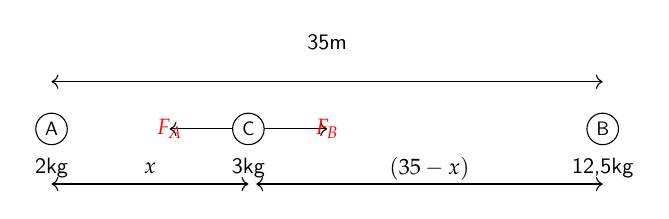
\begin{tikzpicture} 

  \foreach \x/\y/\z in {0/A/{2kg},2.5/C/{3kg},7/B/{12,5kg}} {
    \draw (\x,0) circle (0.2) node[scale=0.7] {\y};
  \node at (\x,-0.5) [scale=0.8]{\z};}
  \draw [<->] (0,0.6)--node [midway, yshift=0.5cm,scale=0.8]{35m}(7,0.6);
  \draw[<->] (0,-0.7) --node [midway, yshift=0.2cm,scale=0.8]{$x$}(2.5,-0.7);
    \draw[<->] (2.6,-0.7) --node [midway, yshift=0.2cm,scale=0.8]{$(35-x)$}(7,-0.7);
    \draw [->] (2.3,0) -- (1.5,0) node [scale=0.8, red]{$F_A$};
        \draw [->] (2.7,0) -- (3.5,0) node [scale=0.8, red]{$F_B$};
    \end{tikzpicture}
  
  Agar total gayanya nol maka besar gaya $F_A$ dan $F_B$ harus sama
  \begin{align*}
  F_A &= F_B\\
  \coret{G}\frac{m_A\coret{m_c}}{x^2} &=\coret {G}\frac{m_B.\coret{m_c}}{(35-x)^2}\\
  \frac{m_A}{m_B} &= \left (\frac{x}{35-x}\right)^2 \\
  \frac{2}{12,5}  &= \left (\frac{x}{35-x}\right)^2 \\
\frac{4}{25}   &= \left (\frac{x}{35-x}\right)^2 \\
\frac{2}{5}&=\frac{x}{35-x}\\
x&= 10 \text{ m dari A}
    \end{align*}
  }






	
% no 5 ---------------------------------------------------------------------------
\item Tiga buah benda masing-masing 1kg, jika jarak A dan B 1m, B dan C 1 m, dan B ada di siku-siku. Maka besar gaya di C  adalah . 
\pilgani{
    \item $\sqrt{2}$ G
    \item $\sqrt{2+\sqrt{2}}$ G
    \item $\sqrt{3}$ G
    \item $ 2 \sqrt{2}$ G
    \item [\kunci{E.}] $\frac{1}{2} \sqrt{5+2\sqrt{2}}$ G
}
\hide{
Cara terbaik mengerjakan soal ini adalah dengan menggambar masing-masing benda dan gaya pada titik C. 

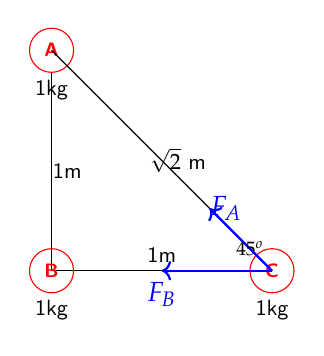
\begin{tikzpicture}[scale=1.4]
\draw [-] (0,1.8)--node [midway, xshift=0.2cm,scale=0.8]{1m}(0,0) -- node [midway, yshift=0.2cm,scale=0.8]{1m}(2,0);
\foreach \x/\y/\name/\mass in {0/2/A/{1kg},0/0/B/{1kg},2/0/C/{1kg}}{
 \draw[red] (\x,\y) circle (0.2) node[scale=0.7] {\textbf{\name}};
 \node at (\x,\y) [yshift=-0.5cm, scale=0.8]{\mass};
 }
 \draw [-](2,0) -- node [midway,xshift=0.2, xshift=0.2cm,scale=0.8]{$\sqrt{2}$ m} (0,2) ;
 \draw [thick,blue,->] (2,0) -- +(135:0.8cm) node[xshift=0.3, xshift=0.2cm] {$F_A$};
  \draw [thick,blue,->] (2,0) --+(180:1cm) node[yshift=-0.3cm] {$F_B$};
  \node at (1.8,0.2)[scale=0.7]{$45^o$};
\end{tikzpicture} 
\begin{align*}
F_c &= \vec{F_A} +\vec{ F_B}\\
\phantom {a}\\
F_A &= G\frac{1.1}{(\sqrt{2})^2} = \frac{1}{2} G\\
F_B &= G\frac{1}{1}{1^2} = G\\
\phantom {a}\\
\end{align*}
}
\hide{
\begin{align*}
F_c &=\sqrt{ F_A^2 +F_B^2 +2.F_A.F_B.\cos \theta  } \\
F_c &=\sqrt{ 1^2 +(\frac{1}{2})^2 +2.1.\frac{1}{2}.{1}{2}\sqrt{2}  } \\
F_c &=\sqrt{\frac{5+2\sqrt{2}}{4}} \\
\end{align*}}







% no 6  ---------------------------------------------------------------------------
\item Benda A massanya 6 kg, benda B 2 kg dan C 4 kg. Jarak A dan B 2 m, jarak B dan C adalah 2 m. Jika B ada di siku-siku maka gaya di titik B adalah . . . .
\pilgani{
	\item[\kunci{A.}] $\sqrt{13} $G N
	\item $2\sqrt{2} $ G N
	\item $ \sqrt{7} $ G N
	\item $ 2\sqrt{3} $ G N
	\item $ 3 $ G  N }
\hide{
langkah pertama mengerjakan adalah mengambar posisi benda

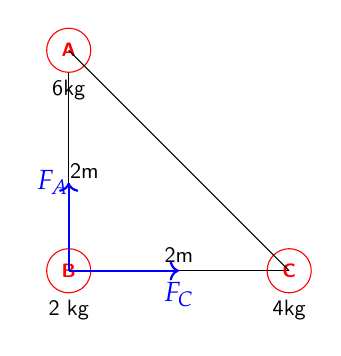
\begin{tikzpicture}[scale=1.4]
\draw [-] (0,1.8)--node [midway, xshift=0.2cm,scale=0.8]{2m}(0,0) -- node [midway, yshift=0.2cm,scale=0.8]{2m}(2,0);
\foreach \x/\y/\name/\mass in {0/2/A/{6kg},0/0/B/{2 kg},2/0/C/{4kg}}{
 \draw[red] (\x,\y) circle (0.2) node[scale=0.7] {\textbf{\name}};
 \node at (\x,\y) [yshift=-0.5cm, scale=0.8]{\mass};
 }
 \draw [-](2,0) -- (0,2) ;
 \draw [thick,blue,->] (0,0) -- +(90:0.8cm) node[xshift=-0.4cm, xshift=0.2cm] {$F_A$};
  \draw [thick,blue,->] (0,0) --+(0:1cm) node[yshift=-0.3cm] {$F_C$};
\end{tikzpicture} 
\begin{align*}
F_{r} &= \vec{F_A} + \vec{F_C} \\
F_r &= \sqrt{F_A^2+F_C^2}\\
\phantom{a}\\
F_A &= G\frac{m_Am_B}{r^2} = G\frac{6.2}{2^2} = 3G\\
F_C &= G\frac{m_Bm_C}{r^2} = G\frac{2.4}{2^2}=2G\\
F_r&=G\sqrt{3^2+2^2} = \sqrt{13} G \text{ N}
\end{align*}
}











%-----------------------------------------
\item [B.18] Tiga bola dengan $m_1$ = 2 kg, $m_2$ = 3 kg, dan $m_3$ = 6 kg ditempatkan pada koordinat (0,-6), (0,0), dan (8,0). Resultan yang dialami oleh massa $m_2$ adalah . . . .
\pilgani{
	\item 1,11 $\times 10^{-11}$ N
	\item 1,88 $\times 10^{-11}$ N
	\item 2,20 $\times 10^{-11}$ N
	\item 2,42 $\times 10^{-11}$ N
	\item [\kunci{E.}]3,92 $\times 10^{-11}$ N
	}
\hide{
	\begin{tikzpicture}[scale=1]
\draw [<->](-0.3,0)--(4.3,0);
\draw [<->] (0,-3.5)--(0,1.5);
\foreach \x/\y/\name/\mass in {0/-3/{$m_1$}/{1kg},0/0/{$m_2$}/{1kg},4/0/{$m_3$}/{1kg}}{
 \draw[red!10!black,fill] (\x,\y) circle (0.1) node[yshift=-0.5cm,xshift=0.5cm] {\textbf{\name}};
 }
 

 \draw [very thick,blue,->] (0,0) -- +(0:2.5cm) node[xshift=0.3, yshift=0.2cm] {$F_3$};
  \draw [very thick,blue,->] (0,0) --+(270:2cm) node[xshift=-0.3cm] {$F_1$};

\end{tikzpicture} 
\begin{align*}
F_2 &= \vec{F_1} + \vec{F_2}\\
\phantom{a}
F_1 & =  G\frac{m_1m_2}{6^2} =G\frac{6}{36}=G\frac{1}{6}\\
F_3 & =  G\frac{m_3m_2}{8^2} =G\frac{36}{64}=G\frac{9}{16}\\
\phantom{A}\\
F_2 &=G \sqrt{ \frac{1}{6}^2+\frac{9}{16}^2   } =G\sqrt{\frac{1}{36} + \frac{9}{16}^2} \\
F_2 &= 3,92 \times 10 ^{-11} \text{ N}
\end{align*}
}




%  ---------------------------------------------------------------------------
\item [B.17] Sebueh benda bermassa 10 kg dibawa ke ketinggian 130 km di atas permukaan Bumi. Jika jari-jari Bumi 6.370 km, berat benda itu pada ketinggian tersebut adalah . . . 
\pilgani{
	\item 93 N
	\item 94 N
	\item 95 N
	\item [\kunci{D.}]96 N
	\item 97 N }
\hide{
	Pada saat di jari-jari, suatu benda mendapatkan medan gravitasi atau percepatan gravitasi $g$ = 10 m/s$^2$. Maka pada ketinggian yang jauh dari permukaan percepatan gravitasinya lebih rendah dengan hubungan
	\begin{align*}
	\frac{g_2}{g_1} &= \frac{\coret{M}}{\coret{M}}\left(\frac{r_1}{r_2} \right)^2\\
	g_2 & = \left(\frac{6370}{6500} \right)^2 g_1 =\left(\frac{49}{50} \right)^2 \times 10\\
	\phantom{2}\\
	w_2&=10.g_2 = 100 \left(\frac{49}{50} \right)^2 = 96 \text{ N}
	\end{align*}
}











% BUKU  20   ---------------------------------------------------------------------------
\item [B.20] Dua buah bola bermassa $m$ dan 4$m$ masing-masing diletakkan pada jarak sejauh $l$. Jika kuat medan gravitasi oleh setiap bola di titik B bernilai sama, jarak AB adalah . . .
\pilgani{
	\item $\frac{l}{9} $
	\item $\frac{l}{6}$
	\item [\kunci{C.}] $\frac{l}{3}$
	\item $\frac{l}{2}$
	\item $\frac{l}{2}$
	}
\hide{
	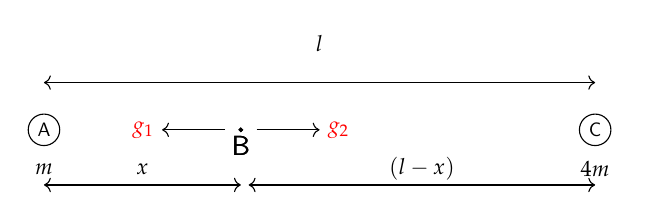
\begin{tikzpicture} 

  \foreach \x/\y/\z in {0/A/{$m$},7/C/{$4m$}} {
    \draw (\x,0) circle (0.2) node[scale=0.7] {\y};
    \draw[fill] (2.5,0) circle (0.021) node [yshift=-0.2cm]{B};
  \node at (\x,-0.5) [scale=0.8]{\z};}
  \draw [<->] (0,0.6)--node [midway, yshift=0.5cm,scale=0.8]{$l$}(7,0.6);
  \draw[<->] (0,-0.7) --node [midway, yshift=0.2cm,scale=0.8]{$x$}(2.5,-0.7);
    \draw[<->] (2.6,-0.7) --node [midway, yshift=0.2cm,scale=0.8]{$(l-x)$}(7,-0.7);
    \draw [->] (2.3,0) -- (1.5,0) node [scale=0.8, red, xshift=-0.3cm]{$g_1$};
        \draw [->] (2.7,0) -- (3.5,0) node [scale=0.8, red,xshift=0.3cm]{$g_2$};
    \end{tikzpicture}
 \begin{align*}
     \frac{x}{l-x}&=\sqrt {\frac{m}{4m}}\\
     2x &= l - x\\
     3x &= l\\
     x &=\frac{l}{3}
     \end{align*}

	}
	
	
	
	
% BUKU 7   ---------------------------------------------------------------------------
\item[B.7] Pada titik titik sudut sebuah segitiga sama sisi dengan panjang sisi $a$ masing-masing ditempatkan benda bermassa $m$. Jika konstanta gravitasi umum $G$, kuat medan gravitasi di pusat segitiga adalah . . . .
\pilgani{
	\item $3G\frac{m}{a^2}$
	\item $G\frac{m}{3a^2}$
	\item $\frac{3}{2}G\frac{m}{a^2}$
	\item $\frac{2}{3}G\frac{m}{a^2}$
	\item [\kunci{E.}] nol}
\hide{

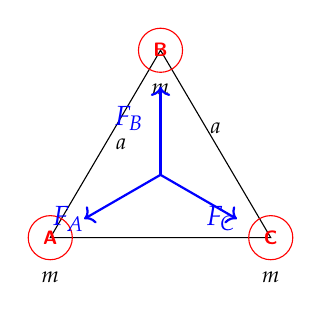
\begin{tikzpicture}[scale=1.4]
\draw [-] (0,0)--node [midway, xshift=0.2cm,scale=0.8]{$a$}(1,1.7) -- node [midway, yshift=0.2cm,scale=0.8]{$a$}(2,0)--cycle;

\foreach \x/\y/\name/\mass in {0/0/A/{$m$},1/1.7/B/{$m$},2/0/C/{$m$}}{
 \draw[red] (\x,\y) circle (0.2) node[scale=0.7] {\textbf{\name}};
 \node at (\x,\y) [yshift=-0.5cm, scale=0.8]{\mass};
 }
 \draw [thick,blue,->] (1,0.57) -- +(90:0.8cm)node[xshift=-0.4cm, yshift=-0.4cm] {$F_B$};
 \draw [thick,blue,->] (1,0.57) -- +(210:0.8cm)node[xshift=-0.4cm, xshift=0.2cm] {$F_A$};
 \draw [thick,blue,->] (1,0.57) -- +(-30:0.8cm)node[xshift=-0.4cm, xshift=0.2cm] {$F_C$};

\end{tikzpicture} 


}






%  BUKU  ---------------------------------------------------------------------------
\item[B.4] Pada setiap titik sudut sebuah segitiga sama sisi dengan panjang sisi $a$ terdapat partikel bermassa $m$. Bersar gaya gravitasi tiap partikel adalah . . . 
\pilgani{
	\item $G\frac{m^2}{a^2}$
	\item $G\frac{m^2}{a^2}\sqrt{2}$
	\item $G\frac{m^2}{a^2}\sqrt{3}$
	\item $2G\frac{m^2}{a^2}$
	\item $G\frac{m^2}{2a^2}\sqrt{3}$}
	
\hide{

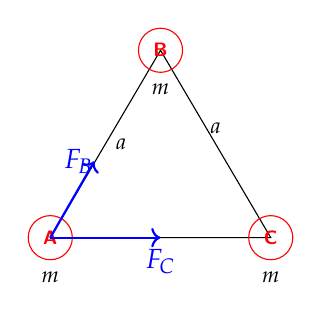
\begin{tikzpicture}[scale=1.4]
\draw [-] (0,0)--node [midway, xshift=0.2cm,scale=0.8]{$a$}(1,1.7) -- node [midway, yshift=0.2cm,scale=0.8]{$a$}(2,0)--cycle;

\foreach \x/\y/\name/\mass in {0/0/A/{$m$},1/1.7/B/{$m$},2/0/C/{$m$}}{
 \draw[red] (\x,\y) circle (0.2) node[scale=0.7] {\textbf{\name}};
 \node at (\x,\y) [yshift=-0.5cm, scale=0.8]{\mass};
 }
 \draw [thick,blue,->] (0,0) -- +(60:0.8cm)node[xshift=-0.4cm, xshift=0.2cm] {$F_B$};
  \draw [thick,blue,->] (0,0) --+(0:1cm) node[yshift=-0.3cm] {$F_C$};
\end{tikzpicture} 


}

\end{enumerate}

%===================================================================
\textbf{B. Perbandingan medan/percepatan, dan berat}
\begin{enumerate}
%no B.1
\item Berat di bumi adalah 3200N. Berat benda tersebut jika berada pada ketinggian $3R$ adalah. . . . \pilgani{
    \item 6400 N
    \item 3200 N
    \item 1600 N
    \item 160 N
    \item 200 N
}
\hide{
Ketinggian $3R$ artinya pada jarak $3R + R = 4R$ dari pusat bumi. Jari $r_2= 4R$. Karena sama-sama terpengaruh bumi (tidak pindah planet, maka $M$ masih sama, yakni $M_{\text{bumi}}$
\begin{align*}
\frac{w_2}{w_1} &= \frac{\coret{G}   \frac{M_2}{r_2^2}} {\coret{G}   \frac{M_1}{r_1^2}} = \frac{M_2}{M_1}\left(\frac{r_1}{r_2}\right)^2\\
\frac{w_2}{3200} &= \frac{\coret{M}}{\coret{M}} \left(\frac{R}{4R}\right)^2 = 200 \text{ N}
\end{align*}

}


%   ---------------------------------------------------------------------------
\item [B.3] Seorang bermassa $m$ berada di permukaan bumi dengan jari-jari bumi $R$ dan massa bumi $M$. Perbandingan gaya gravitasi yang dialami orang ketika berada di permukaan Bumi dan ketika berada pada jarak $R$ di atas permukaan Bumi adalah . . . 
\pilgani{
	\item 1 : 1 
	\item 1 : 2
	\item 2 : 1
	\item 1 : 4
	\item[\kunci{E.}] 4 : 1 }
\hide{
	$r_1$ = $R$ dan $r_2$ berada pada ketinggian $R$ dari permukaan bumi, atau $r_2=2R$ jika dihitung dari pusat (ini yang dipakai)
	\begin{align*}
	F_1 &=G\frac{Mm}{R^2}\\
	F_2 & = G\frac{Mm}{r_2^2}=G\frac{Mm}{2R^2}=\frac{1}{4} F_1\\
	F_1 : F_2 &= 1 : \frac{1}{4} =4 : 1
	\end{align*}
	}



% no B.2   ---------------------------------------------------------------------------
\item Suatu planet mempunyai massa 10 kali bumi dan jari-jari 3 kali bumi. Maka percepatan gravitasi di planet tersebut adalah . . . 
\pilgani{
    \item 2$g$
    \item $\frac{10}{3} g$
    \item $\frac{3}{10} g$
    \item[\kunci{D.}] $\frac{10}{9} g$
    \item $\frac{9}{10} g$
    }
\hide{ 
\begin{align*}
\frac{g_2}{g_1} &= \frac{\coret{G}\frac{M_2}{r_2^2}} {\coret{G} \frac{M_1}{r_1^2}} = \frac{M_2}{M_1}\left(\frac{r_1}{r_2}\right)^2\\
\frac{g_2}{g_1} &=\frac{10}{1}\frac{1}{3^2} \\
{g_2} &= \frac{1}{9}g\\
\end{align*}}








% no B 3 ----------------------------------------------
\item Planet B dengan massa jenis dua kali bumi dan tiga kali jari-jari bumi. Maka percepatan gravitasi di permukan B adalah . . . 
\pilgani{
	\item $ \frac{2}{3} g$
	\item $ \frac{1}{3} g $
	\item $ \frac {3}{1} g $
	\item $ 6 g $
	\item $ 3 g $
	}
\hide{\begin{align*}
\frac{g_2}{g_1} &= \frac{\rho_2 r_2}{\rho_1 r_1} = \frac{2 .3}{1.1}=6\\
g_2 &= 6 g \\
\end{align*}}










% no B 4 ------------------------------------------------
\item Percepatan gravitasi di permukaan bumi adalah 10 N/kg. Pada titik di ketinggian tertentu percepatan gravitasi adalah 2 N/kg. Posisi tersebut dari pusat bumi adalah. . . . 
\pilgani{
	\item[\kunci{A.}]$\sqrt{5}$ R
	\item $\sqrt{2}$ R
	\item $2\sqrt{3}$ R
	\item $2\sqrt{2} $ R
	\item $\frac{1}{2} $ R
	}
\hide{
\begin{align*}
\frac{g_2}{g_1} & = \frac{M_2}{M_1}\frac{r_1^2}{r_2^2}\\
\frac{2}{10} &= \frac{\coret{M}}{\coret{M}}\frac{R^2}{r_2^2}\\
r_2^2 &= 5 R^2 \\
r_2^2 &= \sqrt{5} R\\
\end{align*}}




% No B 5  ---------------------------------------------------------------------------
\item Planet x memiliki percepatan gravitasi 7,5 kali gravitasi bumi. Jika jari-jari planet adalah 2 kali bumi, maka massa planet adalah . . . 
\pilgani{
	\item[\kunci{A.}] $30 M$ 
	\item $20 M $
	\item $10 M$
	\item $ \frac{1}{2} M$
	\item $ \frac{3}{4} M$
	}
\hide{
diketahui $g_2$ = 7,5 kali gravitasi bumi atau 7,5 $g$, dan $r_2$ = 2$r_1$. Massa planet adalah . . . 
\begin{align*}
\frac{g_2}{g_1} & = \frac{M_2}{M_1}\frac{r_1^2}{r_2^2}\\
\frac{7,5}{1} & = \frac{M_2}{M}\frac{r^2}{(2r)^2}\\
7,5 & = \frac{M_2}{4 M}\\
30 M & = M_2
\end{align*}
}







% no B 6 --------------------------------

\item Berat seorang astronot di Bumi adalah 1000 N. Astronot bepergian ke planet X yang mempunyai massa 18 kali bumi dan jari-jari 10 kali bumi. Maka berat astronot tersebut saat berada di ketinggian 2R dari permukaan planet X adalah . . . .
\pilgani {
    \item 3200 N
    \item 3200/9 N
    \item 800 N
    \item 800/3 N
    \item 200 N }
\hide{ 



}


% BUKUUU   ---------------------------------------------------------------------------
\item [B.11] Planet X memiliki massa $a$ kali massa Bumi dan jari-jari $b$ kali bumi. Berat suatu benda di planet X dibandingkan beratnya di  Bumi adalah . . .
\pilgani{
	\item $ab$ kali
	\item $ab^2$ kali
	\item $\frac{a}{b}$ kali
	\item $\frac{a}{b^2}$ kali
	\item $\frac{1}{ab}$ kali }
\hide{

}




% BUKU   ---------------------------------------------------------------------------
\item [B.6] Seorang astronot berada pada orbit lingkaran dengan jari-jari $R$ mengitari Bumi. Agar kuat medan gravitasinya menjadi setengah kali semula, jari-jari lingkaran orbt harus menjadi . . . .
\pilgani{
	\item $\frac{1}{4} R$
	\item $\frac{1}{2} R$
	\item $R\sqrt{2}$
	\item $2R$
	\item $4R$
	}
	
\hide{

}




% BUKU   ---------------------------------------------------------------------------
\item [B.13] Jika jari-jari Bumi adalah $R$ dan medan gravitasi di permukaan Bumi adalah $g$, besarnya medan gravitasi pada ketinggian $h$ dari permukaan Bumi adalah . . 
\pilgani{
	\item $\frac{gh}{R}$
	\item $\frac{gh^2}{(R+h)} $
	\item $\frac{gR^2}{(R+h)}$
	\item $\frac{gh}{(R+h)}$
	\item $\frac{gRh}{(R+h)}$ }
\hide{

}


\end{enumerate}


% ==================================================

\textbf{C. Kecepatan satelit/kecepatan lepas}
\begin{multicols}{2}
\vspace{-0.5cm}
\begin{align*}
v_{satelit} &= \sqrt{\frac{GM}{r}} \\
v_{satelit} &= \sqrt{gr}\\
\end{align*} 

\begin{align*}
v_{lepas} &= \sqrt{\frac{2GM}{r}} \\
v_{lepas} &= \sqrt{2gr}\\
\end{align*} 
\end{multicols}
\vspace{-1.7cm}\begin{align*}
r &= R+h\\
g &= \text{percepatan pada titik tertentu}\\
\end{align*}
Energi Potensial $EP$ dan Potensial $V$
\begin{align*}
EP &= G\frac{Mm}{r}\\
\phantom {s}\\
V &= G\frac{M}{r}\\
\end{align*}

\begin{enumerate}
%no C 1   ---------------------------------------------------------------------------
\item Seorang peneliti berada di planet yang berjari-jari 1000km. Jika percepatan gravitasi di planet adalah 8 m/s$^2$,maka kecepatan minimum untuk lepas dari planet adalah . . . 
\pilgani{
    \item 2 km/s
    \item $\sqrt{8}$ km/s
    \item 4 km/s
    \item 4$\sqrt{10}$km/s
    \item 16 km/s
}
\hide{



}

% no C 2
\item Suatu roket berada di permukaan bumi. Kecepatan minimal agar bisa lepas dari pengaruh gravitasi bumi adalah . . . (R = $6,4 x 10^3$ km)
\pilgani{
	\item $ 8\sqrt{2}$ km/s
	\item $8$ km/s
	\item 16 km/s
	\item 4 km/s
	\item 2 km/s
	}
\hide{



}

% no C 3
\item Suatu planet memiliki massa $2\times 10^{20}$ kg dan jari-jari 1000 km. Maka kecepatan untuk meninggalkan planet adalah . . . . .
\pilgani{
	\item $2\sqrt{G} \times 10^7$ m/s
	\item $\sqrt{G} \times 10^7$ m/s
	\item $\frac{1}{2}\sqrt{G} \times 10^7$ m/s
	\item $\sqrt{2G} \times 10^7$ m/s
	\item $\frac{3}{2}\times 10^7$ m/s
	}
\hide{



}
% no C 4.
\item Pada ketinggian $R$ dari permukaan bumi kecepatan satelit adalah $v$. Apabila satelit berada pada ketinggia $3R$ maka kecepatan satelit mengorbit adalah . . .  
\pilgani{
	\item $\frac{1}{2} v $
	\item $\frac{3}{4} v $
	\item $v$
	\item $2 v$
	\item $\frac{3}{2} $
	}
\hide{


}

\item Suatu roket berada di permukaan planet. Jika roket ingin diluncurkan sampai ketinggian $R$ maka kecepatan yang dibutuhkan adalah . . . 
\pilgani{
    \item $\left ( \frac{4GM}{3R} \right )^{\frac{1}{2}}$
    \item $\left ( \frac{5GM}{3R} \right )^{\frac{1}{2}}$
    \item $\left ( \frac{2GM}{5R} \right )^{\frac{1}{2}}$
    \item $\left ( \frac{GM}{R} \right )^{\frac{1}{2}}$
    \item $\left ( \frac{GM}{3R} \right )^{\frac{1}{2}}$
}
\hide{





}
\end{enumerate}
\textbf{D. Hukum Kepler}

\begin{enumerate}
\item Suatu planet berada pada jarak 2,25 kali jarak bumi matahari. Maka waktu putaran planet tersebut mengelilingi matahari adalah . . . .
\pilgani{
    \item 3,375
    \item 2,25
    \item 1,5
    \item 0,5
    \item 0,25
}
\hide{


}

% D. 2
\item Periode planet A dan B masing-masing 27 dan 8 tahun. Jika diketahui jarak planet B ke pusat tata surya adalah 44 juta km, maka jarak planet A ke pusat tata surya adalah . . . 
\pilgani{
    \item 23
    \item 64
    \item 81
    \item 99
    \item 256
}
\hide{



}

% D 3
\item  Perhatikan pernyataan berikut:
\pernyataan{
    \item Semakin jauh dari pusat matahari, kecepatan planet semakin kecil
    \item Luasan sapuan juring yang sama ditempuh dalam waktu yang sama
    \item Lintasan planet adalah elips dengan matahari di salah satu titik pusatnya
    \item Periode pangkat tiga berbanding lurus dengan jarak ke matahari pangkat dua
}
Pernyataan yang benar tentang hukum Kepler adalah . . .
\pilgani{ 
    \item 1,2,3
    \item 1,3
    \item 2,4
    \item 4 saja
    \item semua benar
}


% Buku
\item [B.10] Jarak rata-rata planet Yupiter dari Matahari adalah 5,2 Satuan Anstronomi. Periode Yupiter mengelilingi Matahari adalah . . . 
\pilgani{
	\item 3,75 tahun
	\item 5,84 tahun
	\item 7,52 tahun
	\item 9,11 tahun
	\item 11,9 tahun}
\hide{

}


%Buku   ---------------------------------------------------------------------------
\item [B.15] Dua satelit beredar mengelilingi Bumi dengan periode tetap. Perbandingan ketinggian kedua satelit dari pusat Bumi 4 : 9. Perbandingan periode kedua satelit tersebut adalah . . 
\pilgani{
	\item 2 : 3
	\item 3 : 2
	\item 4 : 9
	\item 8 : 27
	\item 16 : 91
	}
	
\hide{

}	




\end{enumerate}


\end{multicols*}
\end{document}






